\documentclass{article}

% Language setting
% Replace `english' with e.g. `spanish' to change the document language
\usepackage[english]{babel}

% Set page size and margins
% Replace `letterpaper' with `a4paper' for UK/EU standard size
\usepackage[letterpaper,top=2cm,bottom=2cm,left=3cm,right=3cm,marginparwidth=1.75cm]{geometry}

% Useful packages
\usepackage{amsmath}
\usepackage{graphicx}
\usepackage[colorlinks=true, allcolors=blue]{hyperref}
\usepackage{bm}
\usepackage{tikz}
\usetikzlibrary{fit, positioning}

\usepackage{cleveref}
\crefname{figure}{fig.}{fig.}
\Crefname{figure}{Fig.}{Fig.}
\crefname{equation}{eq.}{eq.}
\Crefname{equation}{Eq.}{Eq.}

\usepackage[color=magenta]{todonotes}



\title{Composition of Movement Primitives}
% \author{Andrea Pierré}

\begin{document}
\maketitle

% \begin{abstract}
% Your abstract.
% \end{abstract}

\tableofcontents

\section{ProMPs}
\subsection{Recap}
From \citep{paraschos_probabilistic_2013, paraschos_using_2018}:
\begin{itemize}
    \item $q_t$: joint angle over time
    \item $\dot{q}_t$: joint velocity over time
    \item $\bm{\tau} = \{q_t\}_{t=0\dots T}$: trajectory
    \item $\bm{w}$: weight vector of a single trajectory
    \item $\phi_t$: basis function
    \item $\bm{\Phi}_t = [\phi_t, \dot{\phi_t}]$: $n \times 2$ dimensional time-dependent basis matrix
    \item $z(t)$: monotonically increasing phase variable
    \item $\bm{\epsilon}_y \sim \mathcal{N}(\bm{0}, \bm{\Sigma}_y)$: zero-mean i.i.d. Gaussian noise
\end{itemize}

\begin{gather}
\bm{y}_t = \begin{bmatrix}
       q_t \\[0.3em]
       \dot{q}_t
     \end{bmatrix} = \bm{\Phi}^{\top}_{t}\bm{w} + \bm{\epsilon}_y\\
p(\bm{\tau}|\bm{w}) = \prod_t \mathcal{N}\Big(\bm{y}_t|\bm{\Phi}^{\top}_{t}\bm{w}, \bm{\Sigma}_y \Big)\\
p(\bm{\tau};\bm{\theta}) = \int p(\bm{\tau}|\bm{w}) \cdot p(\bm{w};\bm{\theta}) d\bm{w}\label{eq:HBM}
\end{gather}

\subsection{Coupling between joints}

\begin{equation}
p(\bm{y}_t|\bm{w}) = \mathcal{N}\Bigg(
        \begin{bmatrix}
                \bm{y}_{1,t} \\
                \vdots\\
                \bm{y}_{d,t} \\
        \end{bmatrix}
        \Bigg|
        \begin{bmatrix}
                \bm{\Phi}^{\top}_{t} & \cdots & \bm{0} \\
                \vdots &\ddots & \vdots\\
                \bm{0} & \cdots & \bm{\Phi}^{\top}_{t} \\
        \end{bmatrix}
        \bm{w}, \bm{\Sigma}_y
\Bigg) = \mathcal{N}\Big(\bm{y}_t|\bm{\Psi}_t\bm{w},\bm{\Sigma}_y \Big)
\end{equation}

with:
\begin{itemize}
    \item $\bm{w}=[\bm{w}^\top_1, \dots, \bm{w}^\top_n]^\top$: combined weight vector
    \item $\bm{\Phi}_t$: block-diagonal basis matrix containing the basis functions and their derivatives for each dimension
    \item $\bm{y}_{i,t} = [q_{i,t}, \dot{q}_{i,t}]^\top$: joint angle and velocity for the $i^{\text{th}}$ joint
\end{itemize}

\subsection{Hierarchical Bayesian Model}

The Hierarchical Bayesian Model used in ProMPs is illustrated in \Cref{fig:HBM}.

\begin{figure}[htbp]
\centering
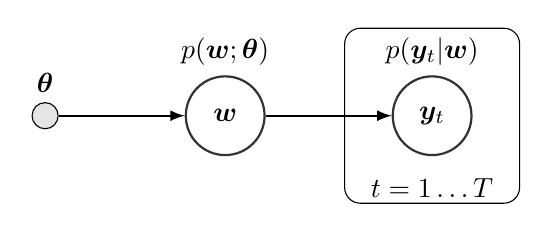
\begin{tikzpicture}
\tikzstyle{main}=[circle, minimum size = 10mm, thick, draw =black!80, node distance = 16mm]
\tikzstyle{connect}=[-latex, thick]
\tikzstyle{box}=[rectangle, draw=black!100]
  \node[circle, draw=black!100, fill = black!10] (theta) [label=above:$\bm{\theta}$] { };
  \node[main] (w) [right=of theta,label=above:$p(\bm{w};\bm{\theta})$] {$\bm{w}$};
  \node[main] (y) [right=of w,label=above:$p(\bm{y}_t|\bm{w})$] {$\bm{y}_t$};
  \path (theta) edge [connect] (w)
		(w) edge [connect] (y);
  \node[rectangle, inner sep=1.5mm, fit= (y),label=below:{$t=1 \dots T$}] (ghost) {};
  \node[rectangle, rounded corners=0.2cm, inner sep=4.4mm,draw=black!100, fit= (y) (ghost)] {};
\end{tikzpicture}
\caption{Hierarchical Bayesian Model used in ProMPs.}
\label{fig:HBM}
\end{figure}

\begin{itemize}
  \item $\bm{\theta} = \{\bm{\mu}_{w}, \bm{\Sigma}_{w}\}$
  \item $p(\bm{w};\bm{\theta}) = \mathcal{N}(\bm{w}|\bm{\mu}_{w}, \bm{\Sigma}_{w})$: prior over the weight vector $\bm{w}$, with parameters $\bm{\theta}$, assumed to be Gaussian
\end{itemize}

\begin{align}
p(\bm{y}_t; \bm{\theta}) &= \int \mathcal{N}\Big(\bm{y}_t|\bm{\Psi}^\top_t \bm{w}, \bm{\Sigma}_y \Big) \cdot p(\bm{w}; \bm{\theta}) \; d\bm{w}\\
&= \int \mathcal{N}\Big(\bm{y}_t|\bm{\Psi}^\top_t \bm{w}, \bm{\Sigma}_y \Big) \cdot \mathcal{N}\Big(\bm{w}|\bm{\mu_w}, \bm{\Sigma_w} \Big) \; d\bm{w}\\
&= \textcolor{blue}{ \int \mathcal{N}\Big( \bm{w}|\bm{\Psi}^\top_t \bm{w}, \bm{\Sigma_{w}} + \bm{\Sigma}_{y}  \Big) \; d\bm{w} \quad \text{(product of Gaussian densities)}}\\
& \textcolor{magenta}{\dots\text{Missing development}\dots}\\
&= \mathcal{N}\Big( \bm{y}_t | \bm{\Psi}^\top_t \bm{\mu_w}, \bm{\Psi}^\top_t \bm{\Sigma_w} \bm{\Psi}_t + \bm{\Sigma}_y \Big)
\end{align}

\subsection{Via-Points Modulation}

\begin{itemize}
    \item $\bm{x}_t^\star = [\bm{y}_t^\star, \bm{\Sigma}^\star_t]$: desired observation
    \item $\bm{y}^\star_t$: desired position and velocity vector at time $t$
    \item $\bm{\Sigma}^\star_t$: accuracy of the desired observation
\end{itemize}

Using Bayes rule:
\begin{align}
  p(\bm{w}|\bm{x}_t^\star) &= \frac{p(\bm{x}_t^\star|\bm{w}) \cdot p(\bm{w})}{p(\bm{x}_t^\star)} \\
  p(\bm{w}|\bm{x}_t^\star) &\propto \mathcal{N}\Big( \bm{y}_t^\star | \bm{\Psi}_t^\top\bm{w}, \bm{\Sigma}^\star_t \Big) \cdot p(\bm{w})\label{eq:prob-cond-new}
\end{align}

From \citep{deisenroth2020mathematics, joram_soch_2025_14646799, bishop2023deep}, the parameters of a conditional multivariate Gaussian $p(\bm{x}|\bm{y}) = \mathcal{N}\big( \bm{\mu}_{x|y}, \bm{\Sigma}_{x|y} \big)$ are the following:
\begin{align}
  % p(\bm{x}|\bm{y}) &= \mathcal{N}\big( \bm{\mu}_{x|y}, \bm{\Sigma}_{x|y} \big)\\
  \bm{\mu}_{x|y} &= \bm{\mu}_{x} + \bm{\Sigma}_{xy}\bm{\Sigma}_{yy}^{-1}(\bm{y} - \bm{\mu}_{y})\\
  \bm{\Sigma}_{x|y} &= \bm{\Sigma}_{xx} - \bm{\Sigma}_{xy}\bm{\Sigma}_{yy}^{-1}\bm{\Sigma}_{yx}
\end{align}

\begin{align}
& \textcolor{magenta}{\dots\text{ToDo expand}\dots}\\
\bm{\mu_w}^{[new]} &= \bm{\mu_w} + \bm{\Sigma_w}\bm{\Psi}_t \Big(\bm{\Sigma}_y^\star \bm{\Psi}_t^\top \bm{\Sigma_w}\bm{\Psi}_t \Big)^{-1} (\bm{y}_t^\star - \bm{\Psi}_t^\top \bm{\mu_w})\label{eq:mu-cond-new}\\
\bm{\Sigma_w}^{[new]} &= \bm{\Sigma_w} - \bm{\Sigma_w}\bm{\Psi}_t \Big(\bm{\Sigma}_y^\star \bm{\Psi}_t^\top \bm{\Sigma_w}\bm{\Psi}_t \Big)^{-1} \bm{\Psi}_t^\top \bm{\Sigma_w}\label{eq:sigma-cond-new}
\end{align}



\section{Composition of MPs}
\todo[inline]{ToDo}




\bibliographystyle{IEEEtranN}
\bibliography{references}

\end{document}
